\section{Implementation}
\subsection{General implementation}
\subsection{Map and flower patch quality}
\subsection{Hives}
\subsection{Scouts}
	\subsubsection{Random walk}
		\begin{figure}\label{fig:randomWalk}
			\centering
			\scalebox{.75}{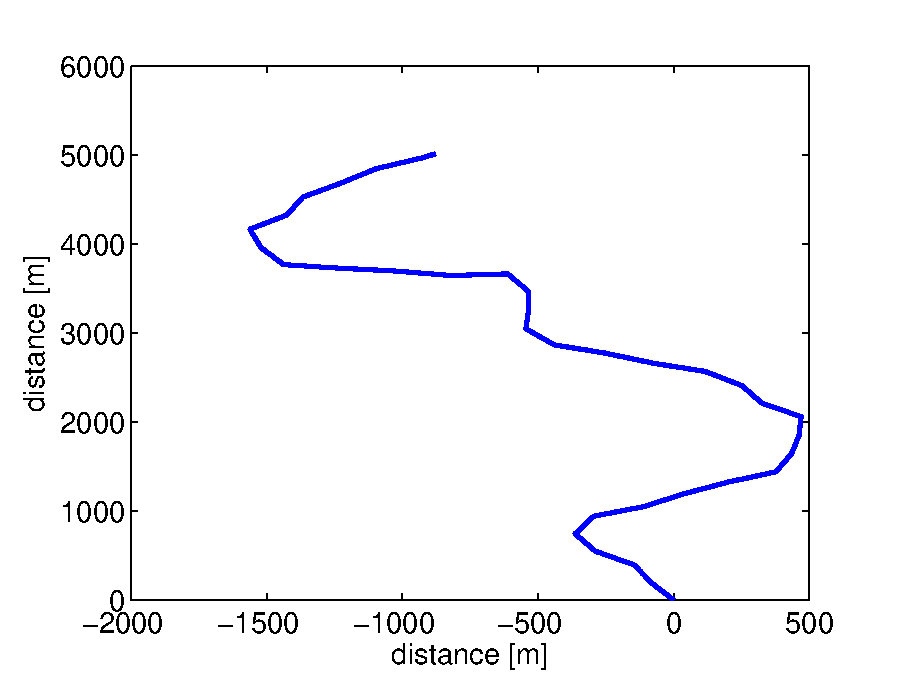
\includegraphics{data/random_walk.eps}}
			\caption{\textit{Example of a random walk executed by a scout bee.}}
		\end{figure}
	\subsubsection{Bresenham line algorithm}

\subsection{Foragers}
	\subsubsection{Path optimization}
		\begin{figure}\label{pathOptimization}
			\centering
			\scalebox{.75}{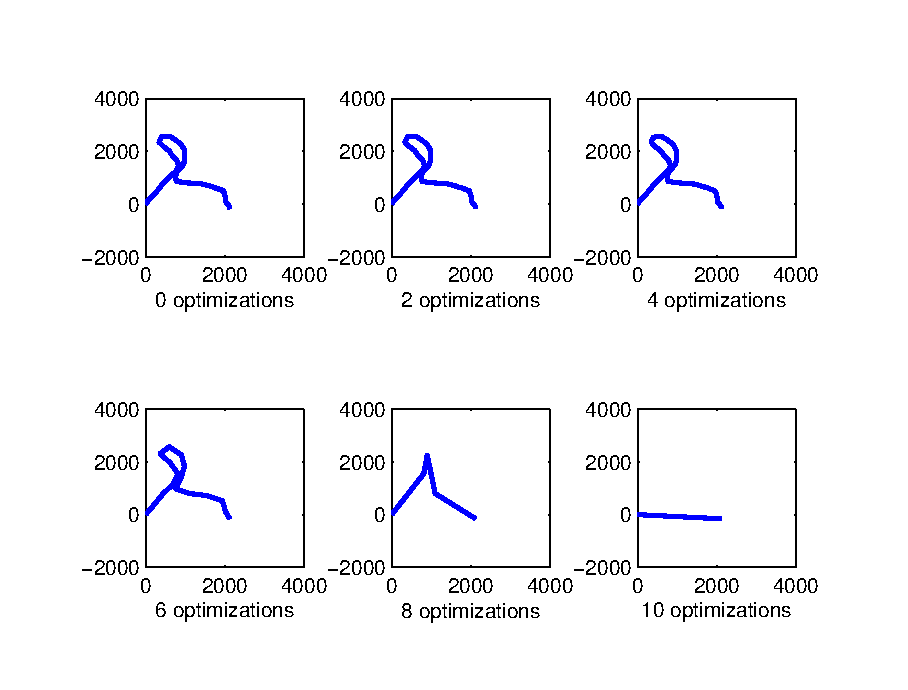
\includegraphics{data/optimization.eps}}
			\caption{\textit{Example of path optimization used to short cut the path to flower patches.}}
		\end{figure}